\section{Mechanistic Workload Analysis (RQ3, part 2)}
\label{sec:mechanisms}

Sections~\ref{sec:characterization} and~\ref{sec:linkage} show
\emph{that} discriminativeness and offline$\leftrightarrow$closed-loop
agreement vary by workload; this section asks \emph{why}, using only
existing trace-only and closed-loop artifacts (no new simulation). Source:
repository path
\texttt{analysis/\allowbreak closed\_\allowbreak loop\_\allowbreak mechanistic\_\allowbreak analysis\_\allowbreak 20260914/}.
Classifications follow the source report's own discipline exactly:
\textsc{directly observed} (a deductive or exactly-reproduced fact),
\textsc{consistent with mechanism} (plausible, structurally supported, not
proven), and \textsc{causally established} (reserved for one deductive
result below). No claim here is upgraded beyond its source classification.

\textbf{Capacity-scale reuse correlates with both discriminativeness and
closed-loop separation.} Trace-derived LRU hit rate (an exact,
capacity-scale reuse measure, computed independently of the labels)
correlates with offline discriminativeness at $r=0.83$ and with
closed-loop $|\text{MRU}-\text{LRU}|$ separation at $r=0.90$ (pooled
$n=10$). Figure~\ref{fig:locality} shows both relationships directly.
This is an $n=10$, exploratory finding, consistent with but not
independent evidence from RQ-CL3's own exploratory correlation
(Section~\ref{sec:linkage}) -- the same underlying trace property is
driving both.

\begin{figure}[t]
  \centering
  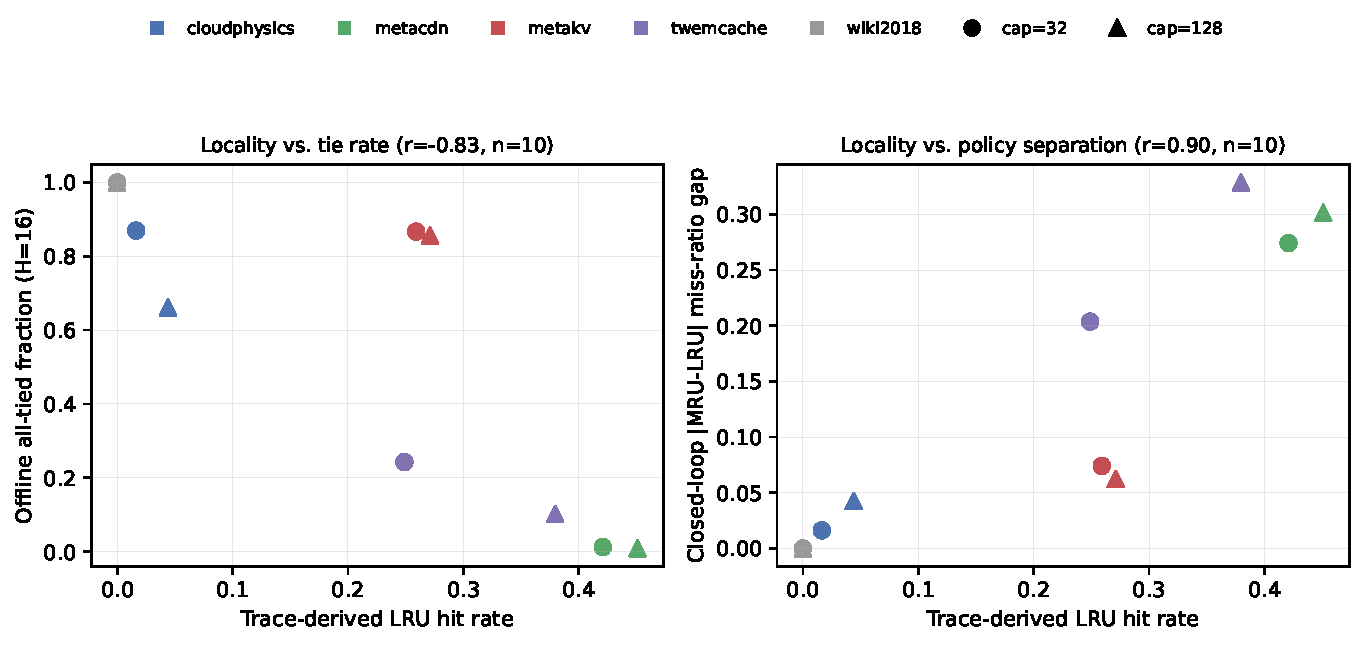
\includegraphics[width=\columnwidth]{figures/figure4_locality.pdf}
  \caption{Trace-derived LRU hit rate vs.\ offline discriminativeness
  (left) and closed-loop policy separation (right), $n=10$ family$\times$capacity
  cells. Reproducible from
  \texttt{paper/performance\_evaluation/scripts/figures/make\_figure4\_locality.py}
  against \texttt{outputs/mechanism\_comparison.csv}.}
  \label{fig:locality}
\end{figure}

\textbf{alibaba-block/cap32 is near-zero signal.} Only 17.5\% of window requests are
reuses at all; of those, only 9.4\% fall within stack distance 32. The
trace-only predicted LRU hit rate ($0.175 \times 0.094 = 1.6\%$) exactly
reproduces the observed Tier-1 LRU hit rate (134/8192 = 1.64\%). The
offline regret gaps there ($-0.0027$, $-0.0007$) are tiny on a scale where
metacdn's own MRU-LRU gap is over 100$\times$ larger. The
Section~\ref{sec:linkage} discordance at this cell is exactly what a
coin-flip-scale signal would produce.

\textbf{metakv/cap128 remains a bounded exception.} metakv's reuse-distance median is short (2, comparable to
metacdn's 3) but its tail is markedly heavier: reuse-within-32 is only
0.574, rising to just 0.600 by distance 128 -- a narrow, 2.6-percentage-point
``boundary zone'' sitting almost exactly at the tested capacities, where a
recency-strict policy (LRU) and a second-chance policy (SIEVE) can
plausibly diverge. metakv's cold-start scoring window
(Section~\ref{sec:experimental-methodology}) is a second, independently
real structural property of this same cell. \textbf{Neither is shown to be
the cause}: no per-request SIEVE or random trajectory log exists in the
frozen artifacts to isolate which property (or their interaction, or
neither) produced the reversal, and the source analysis states this
explicitly rather than forcing a resolution.

\textbf{twemcache's random-over-SIEVE ordering is not explained by
existing data.} twemcache has the strongest ``small hot set plus long
tail'' bimodal signature in the dataset (longest novel streak 3; reuse
distance p10=3 but p75=7379), which would naively predict SIEVE's
second-chance admission should help -- but the observed result is the
opposite (SIEVE loses to random at both capacities). Existing trace-only
data can describe this structure but cannot explain the direction of the
outcome; the source analysis classifies any ``SIEVE benefits from
bimodality'' story here as \textsc{not supported} by the data, and this
paper does not repeat that story.

\textbf{wiki2018 (\textsc{causally established}): the one exception to the
paper's general classification discipline, and deliberately so.} Zero
reuse events occur in the scored window ($n_{\text{reuse}}=0$ across all
4096 requests, every one a first-ever occurrence over the full 50{,}000-request
trace). Since a hit requires a repeated reference to an already-resident
item, miss ratio $=1.0$ for every policy is a mathematical certainty given
zero reuse events, not a statistical tendency -- an existence proof from a
directly counted quantity, which is why this one result is classified
\textsc{causally established} while every other mechanism in this section
is not.
